\subsection{Compare Boundaries Stats}\label{HiC:compare-boundaries-stats}% __12b-compare-boundaries-stats
%~~~~~~~~~~~~~~~~~~~%
\subsubsection{Input} % inputs
Data from the pipeline \texttt{compare-boundaries} step is used as input (Section~\ref{HiC:compare-boundaries}).
%~~~~~~~~~~~~~~~~~~~%
\subsubsection{Analysis} % analysis
Default parameters:
\begin{lstlisting}
params.standard.tcsh$
#!/bin/tcsh

source ./inputs/params/params.tcsh
\end{lstlisting}
%~~~~~~~~~~~~~~~~~~~%
\subsubsection{Output} % outputs
See Figure~\ref{fig:compare-boundaries-stats_correlograms} and Figure~\ref{fig:compare-boundaries-stats_raw_comparisons}. Default output:
\begin{lstlisting}
-rw-r--r-- 1 at570 6.9K Feb 12 12:52 comparisons.tsv
-rw-r--r-- 1 at570  27K Feb 12 12:52 correlograms.pdf
-rw-r--r-- 1 at570  238 Feb 12 12:52 job.err
-rw-r--r-- 1 at570   47 Feb 12 12:51 job.id
-rw-r--r-- 1 at570   52 Feb 12 12:52 job.out
-rw-r--r-- 1 at570 3.5K Feb 12 12:51 job.sh
-rw-r--r-- 1 at570  51K Feb 12 12:52 job.vars.tsv
-rw-r--r-- 1 at570 5.6K Feb 12 12:52 raw_comparisons.pdf
\end{lstlisting}
\begin{figure}[!htb]
    \centering
    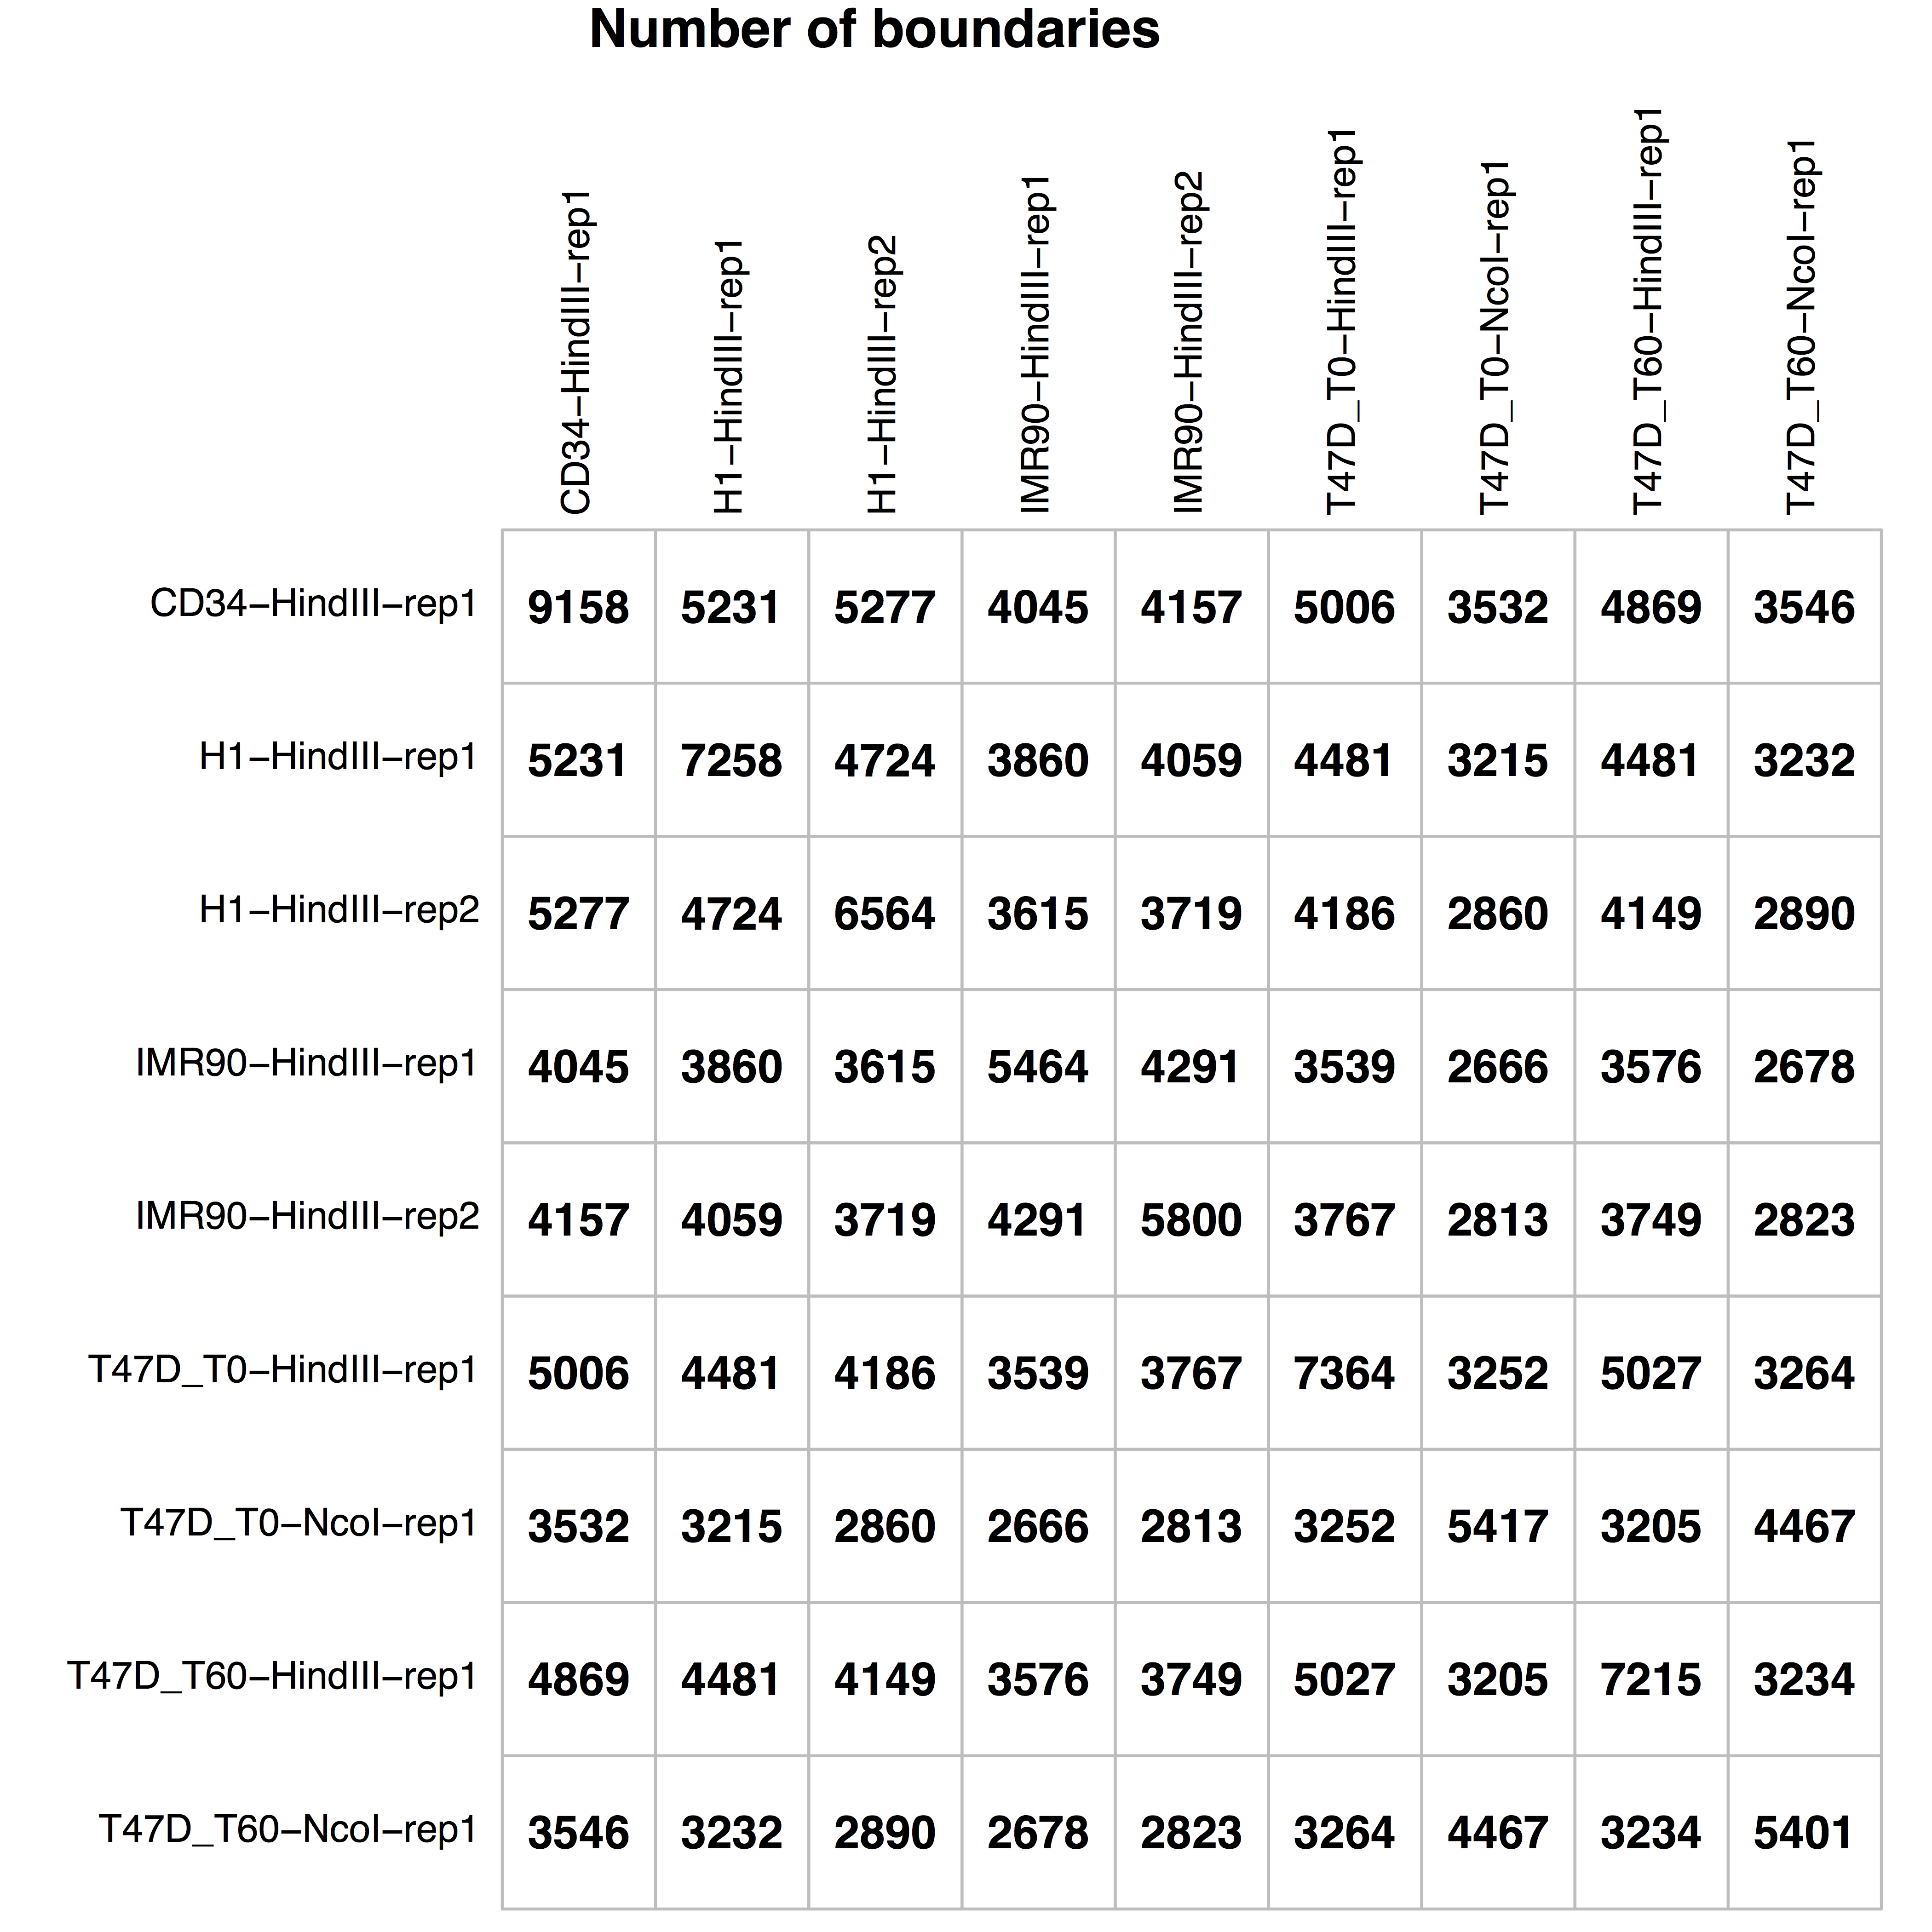
\includegraphics[width=\textwidth,height=\textheight,keepaspectratio]{figure/compare-boundaries-stats_raw_comparisons}
    \caption{Example raw comparisons. See Section~\ref{HiC:compare-boundaries-stats}.} % results/compare-boundaries-stats.standard/compare-boundaries.by_sample.standard/domains.by_sample.armatus.gamma_0.5/matrix-filtered.by_sample.res_40kb/filter.by_sample.standard/align.by_sample.bowtie2/hg19/all-samples/raw_comparisons.pdf
    \label{fig:compare-boundaries-stats_raw_comparisons}
\end{figure}

\begin{figure}[!htb]
    \centering
    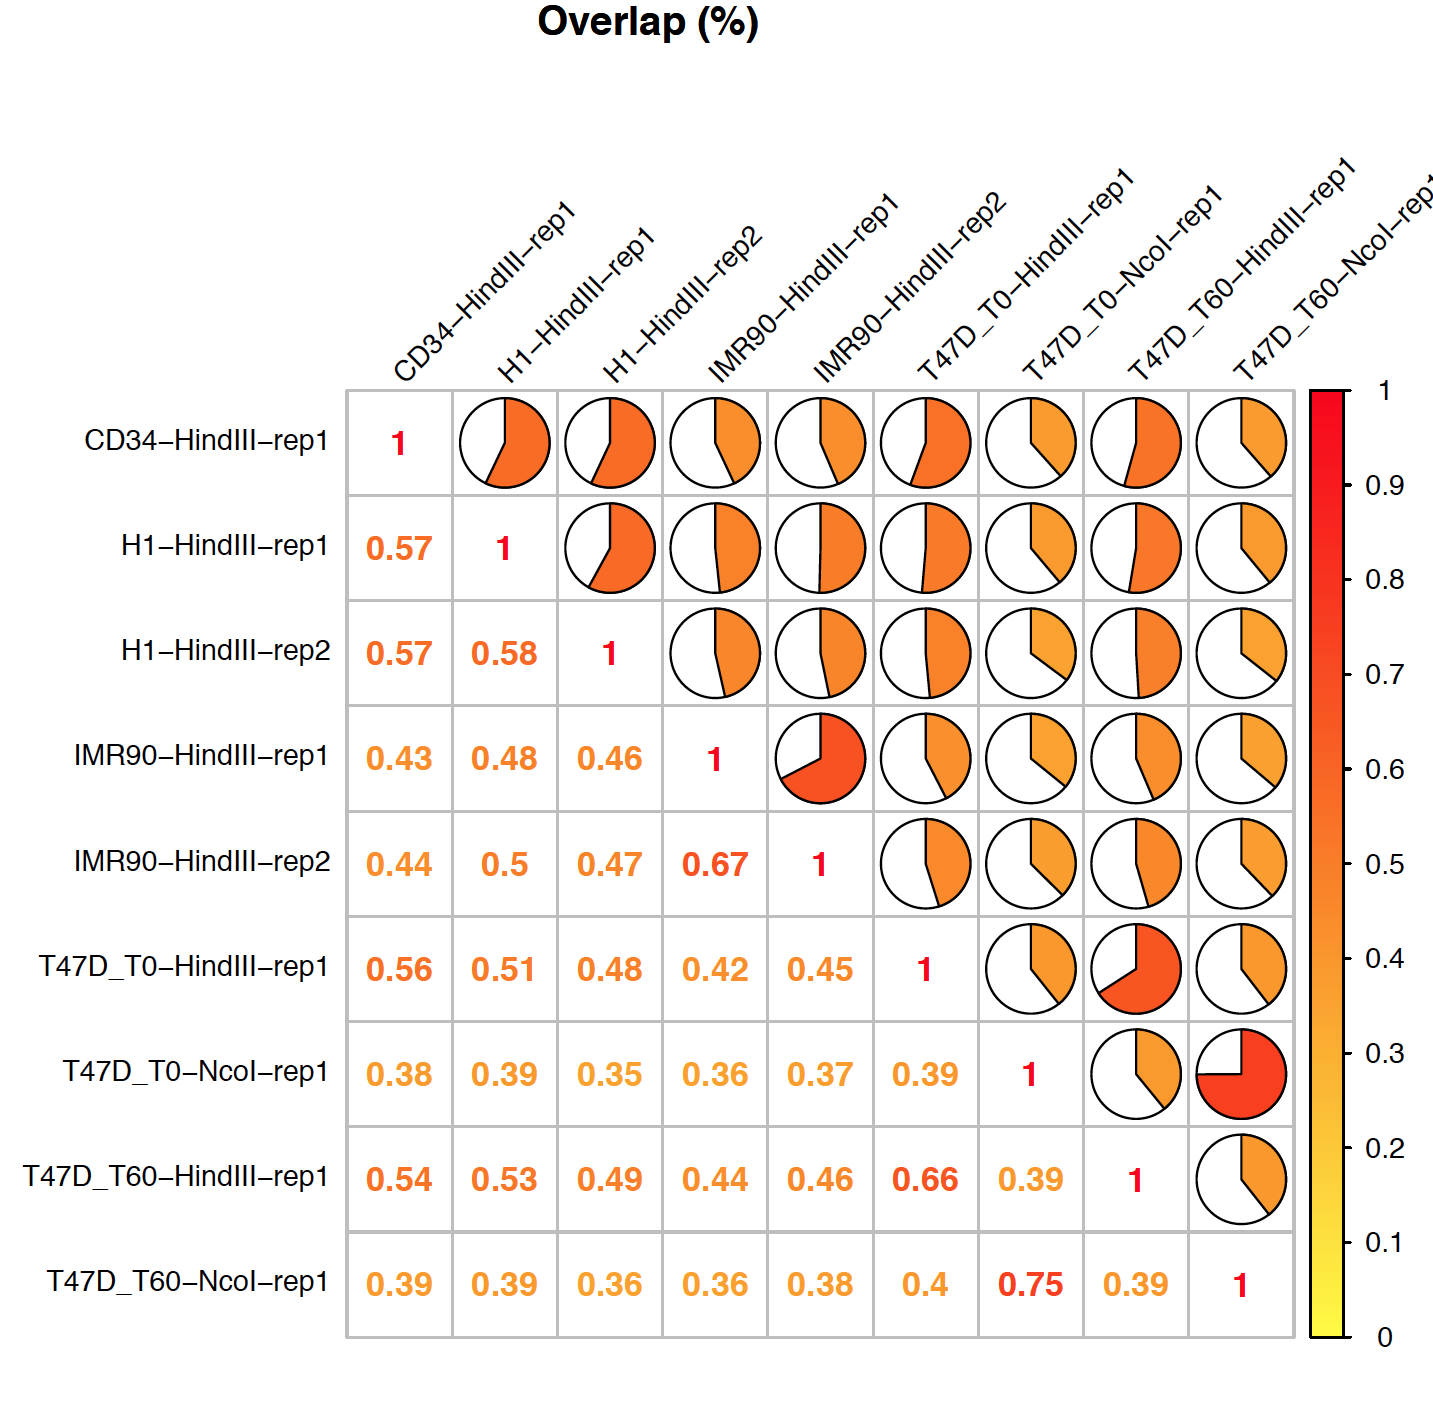
\includegraphics[width=\textwidth,height=\textheight,keepaspectratio]{figure/compare-boundaries-stats_correlograms}
    \caption{Example correlograms. See Section~\ref{HiC:compare-boundaries-stats}.} % results/compare-boundaries-stats.standard/compare-boundaries.by_sample.standard/domains.by_sample.armatus.gamma_0.5/matrix-filtered.by_sample.res_40kb/filter.by_sample.standard/align.by_sample.bowtie2/hg19/all-samples/correlograms.pdf
    \label{fig:compare-boundaries-stats_correlograms}
\end{figure}
% \newpage
\clearpage